\section{Experimental Data}
\label{sec:data}

    We generated several problem suites with \fuzzer{} that made one solver perform poorly, but not others. These suites are \theSuites{}. Figure~\ref{fig:cvc-hard} shows the suites that were uniquely difficult for \cvc{}. Figure~\ref{fig:z3str3-hard} shows the suites that were uniquely difficult for \us{}. All experiments were run in series on the same Linux computer, with a timeout of 15 seconds.

    \begin{figure}[H]
        \begin{subfigure}{.5\textwidth}
            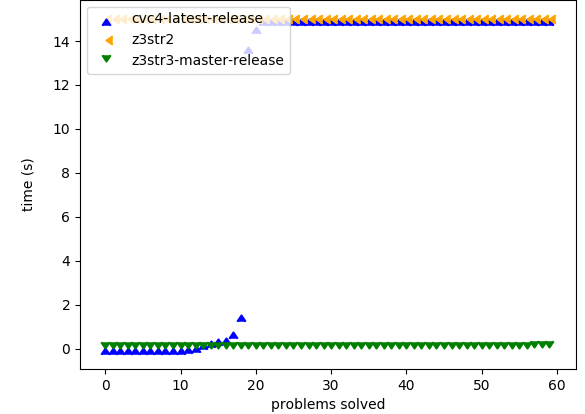
\includegraphics[width=\textwidth]{data/graphs/concats-extracts-small.png}
            \label{fig:concats-extracts-small}
            \caption{Performance on concats-extracts-small}
        \end{subfigure}
        \begin{subfigure}{.5\textwidth}
            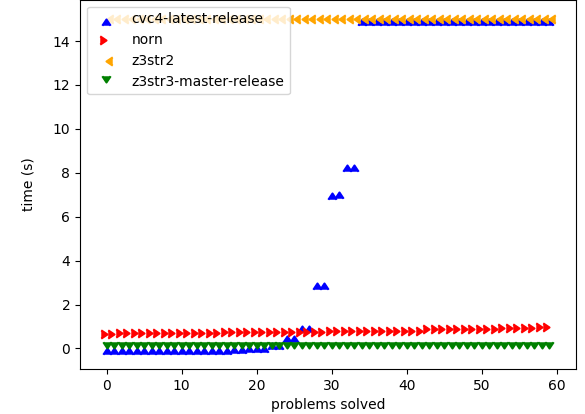
\includegraphics[width=\textwidth]{data/graphs/different-prefix.png}
            \label{fig:different-prefix}
            \caption{Performance on different-prefix}
        \end{subfigure}
        \caption{Problems hard for \cvc{}}
        \label{fig:cvc-hard}
    \end{figure}

    \begin{figure}[H]
        \begin{subfigure}{.5\textwidth}
            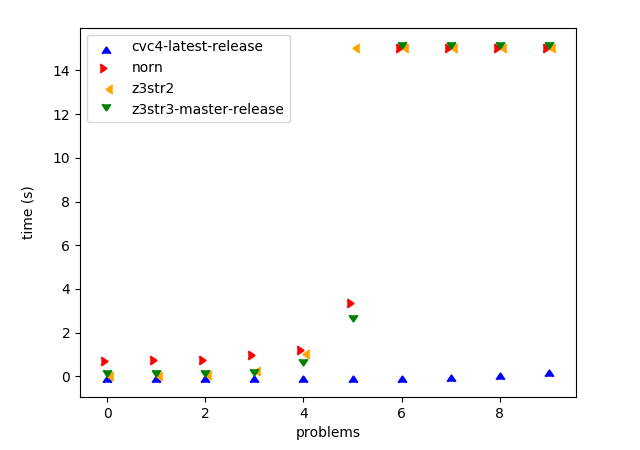
\includegraphics[width=\textwidth]{data/graphs/concats-balanced.png}
            \label{fig:concats-balanced}
            \caption{Performance on concats-balanced}
        \end{subfigure}
        \begin{subfigure}{.5\textwidth}
            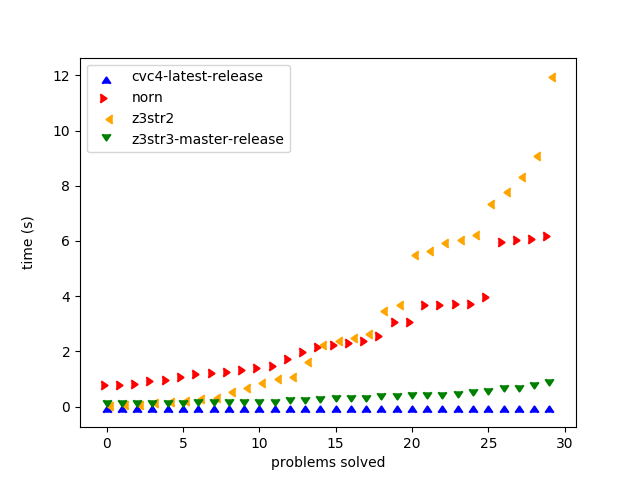
\includegraphics[width=\textwidth]{data/graphs/concats-small.png}
            \label{fig:concats-small}
            \caption{Performance on concats-small}
        \end{subfigure}
        \caption{Problems hard for \us{}}
        \label{fig:z3str3-hard}
    \end{figure}

\section{Analyses}
\label{sec:analysis}

    In this section, we analyse our experimental results. We discuss the causes of \us{}'s poor performance on the two problem suites: \textit{concats-balanced} and \textit{concats-big}. We were not equipped well enough to debug the behaviours of the other solvers, but we provide our data in hopes that they will be useful to the solvers' authors.

    \subsection{\us{} on concats-balanced}

        \todo{Dmitry with help: Explain why \us{} performs poorly on this suite.}

% X = "solution"
% X = (((A.B).(C.D)).((E.F).(G.H))).
%     (((I.J).(K.L)).((M.N).(O.P)))

    \subsection{\us{} on concats-big}

        \todo{Dmitry with help: Explain why \us{} performs poorly on this suite.}

% X = "solution"
% X = (A.(B.(C.(D.(E.(F.(G.H)))))))
